% 
% Pekny den,
% 
% konecne jsem se dostal k precteni textu. Mam v soucasne dobe nasledujici
% poznamky:
% DONE 1) od druheho odstavce kap. 3 bych z toho udelal podkapitolu "UVOD"
% DONE 2) po uvodu bych dal schema blokove a soucasny 4. odstavec trosku rozvedl
% DONE 3) lepe formulovat vsechny instrukce jsou => Instrukce jsou kodovany
% pomoci 16, 32 nebo 48 bitu pricemz operacni kod je situovan vzdy v
% prvnich 16 bitech.
% DONE 4) kap 3 lepe clenit - periferie dat do podkapitoly napr. Zakladni
% periferie; at je z obsahu zrejme, ze se zabyvate IS, periferiemi, apod
% 5) kap 4  by  bylo vhodne prejmenovat, aby bylo zrejme, ze budete
% popisovat obecne platnou zalezitost; nicmene pokud by mel rozsah zustat
% spise maly, lepsi by bylo text pridat do kapitoly zabyvajici se
% navrhem/implementaci ci jinam
% DONE 6) kap 5 - vystizneji nazvat - napr. "Navrh udalostne rizeneho simulatoru"
% DONE 7) Cílem této kapitoly je návrh simulátoru => Cílem této kapitoly je
% popsat strukturu navrzeneho simulatoru
% DONE 8) Pred kapitolu 5 bych dal kapitolu "Udalostne rizena simulace" a do ni
% rozebral a) co to je a b) existujici systemy vcetne DEVS; v kapitole 5
% se jen odkazat,ze to bude vyuzito
% DONE 9) v ramci kap 5 bych asi nazyval komponentu msp430 simulacnim jadrem,
% ale to je spise k diskusi
% DONE 10) kap 5 by mela zacit "Struktura navrzeneho simulatoru", kde by se
% zminilo jadro + rozsireni (podpora pro periferie) + nad tim GUI; teprve
% pote se zabyvat popisem jednotlivych casti
% DONE 11) zatim bych text v kap5 nechal byt a jakmile si budete myslet, ze je
% kompletni, detailne bych jej procetl a napsal pripominky; nyni se mi
% zda, ze tam je spoustu informaci, ale chtelo by je to trosku utribit
%       chtelo by to napsat zminku, ktere mechanismy se budou z DEVS
% pouzivat (nikoliv vsak uplne detaily - ty budou az v implementaci) -
% napr. "Komponenty budou ke komunikaci vyuzivat ...."

\chapter{Úvod}

Mikrokontrolery (MCU) jsou monolitické integrované obvody obsahující mikroprocesor, paměť pro uložení programu, paměť pro jeho běh a další periferie
rozšiřující jeho funkčnost. Vyznačují se jednoduchostí, kompaktností a malou spotřebou. Používají se tak proto především pro jednoúčelová zařízení a 
vestavěné (embedded) systémy.

Při návrhů vestavěných systémů je v praxi často používána simulace. Díky využití simulátoru daného mikrokontroleru (případně celého vestavěného systému) lze ověřit funkčnost systému již při jeho návrhu aniž by bylo nutné vynaložit náklady na prvotní prototypy. Simulační čas lze zrychlit nebo naopak zpomalit a tím jednodušeji prozkoumat vybrané jevy. Simulace může rovněž zjednodušit hledání problémů viděných na reálném hardwaru, kdy jejich příčiny nelze prostým zkoumáním reálného systému jednoduše odhalit. Při použití simulace je také jednodušší vyzkoušet případné změny systému a zkoumat nové postupy bez dalšího zvýšení nákladů. Nejen z těchto důvodů je tedy simulace vestavěných systémů užitečná a má smysl se jí zabývat.

Tato semestrální práce si dává za cíl návrh jednoduše rozšiřitelného pokročilého simulátoru mikrokontrolerů rodiny MSP430 od výrobce Texas Instruments. Tyto mikrokontrolery jsou hojně rozšířené především díky své nízké ceně, malé spotřebě a jednoduchosti práce s nimi. Lze je nalézt například i v platformě FITkit používané k výukovým účelům Fakultou informačních technologií Vysokého učení technického v Brně. Simulátor navrhovaný v této práci je navrhován právě jako doplňující prostředek pro vývoj aplikací pro tuto platformu, avšak bude moci být použit i samostatně. V současné době není obdobný software pod svobodnou licencí dostupný.

% Mikrokontroler MSP430, kterého se táto práce týká, je postaven na von Neumannově architektuře (má tedy společnou paměť pro data i program). Paměť je adresována po bytech složených z 8 bitů a páry bytů tvoří 16bitové little-endian slova.


\chapter{Mikrokontroler MSP430}

Tato kapitola stručně shrnuje základy architektury mikrokontrolerů rodiny MSP430. Nesnaží se však kompletně nahradit jejich dokumentaci, ačkoliv z ní vychází. Pro návrh a implementaci kompletního simulátoru nejsou informace v této kapitole dostačující, ale byly vybrány s ohledem na úvod do problematiky mikrokontrolerů MSP430 a pochopení následujících kapitol a činnosti navrhovaného simulátoru.

\begin{figure}[ht]
\centering
\includegraphics[trim=0cm 0cm 0cm 0cm, scale=0.5]{fig/msp430block}
\caption{Blokové schéma mikrokontroleru MSP430.}
\label{fig:msp430block}
\end{figure}

Mikrokontroler je rozdělen na několik bloků, které lze vidět na obrázku \ref{fig:msp430block}. Jádrem celého mikrokontroleru je 16bitový mikroprocesor
vykonávající instrukce programu definované jeho instrukční sadou. Frekvence mikroprocesoru a všech dalších periferií je řízena systémem hodin (Clock System). K mikroprocesoru je pomocí 16bitové adresové sběrnice a 16bitové datové sběrnice připojena paměť programu (Flash/ROM) a paměť dat (RAM). Další doplňující periferie jsou pak adresovány adresovou sběrnicí o menší šířce v závislosti na modelu mikrokontroleru. Datová sběrnice periferií je buď 16bitová nebo 8bitová v závislosti na potřebě konkrétní periferie.

Jednotlivé bloky mikrokontroleru MSP430 jsou podrobněji popsány dále v této kapitole.

\section{Mikroprocesor a instrukční sada}

Mikrokontrolery rodiny MSP430 obsahují 16bitový mikroprocesor (CPU) a 16 registrů, každý o kapacitě 16 bitů. První čtyři registry mají speciální účel. Registr R0 slouží jako ukazatel na aktuální instrukci (PC - program counter). Register R1 ukazuje na vrchol zásobníku (SP - stack pointer). Register R2 je stavovým registrem (SR - status register) obsahujícím informace o stavu mikroprocesoru. Register R3 je použit pro generování často používaných konstant, takže je není potřeba načítat z paměti. Ostatní registry je možné volně využít v uživatelském programu.

Nejdůležitějšími stavovými bity ve stavovém registru jsou bity N (nastaven pokud je výsledek operace negativní), Z (nastaven pokud je výsledek operace nulový), C (nastaven pokud došlo k přenosu nejvyššího bitu) a V (nastaven pokud došlo při operaci k přetečení).

\subsection{Instrukční sada}

Instrukční sada obsahuje 27 instrukcí. Instrukce jsou kódovány pomocí 16, 32 nebo 48 bitů přičemž operační kód je situován vždy v prvních 16 bitech.

Většina instrukcí pracujících s daty umí pracovat jak s operandem velikosti jednoho bytu, tak s celým slovem. Instrukce lze rozdělit do 3 typů, které se liší i rozdílným kódováním v prvních 16 bitech instrukce uložené v paměti:

\subsubsection{Instrukce s jedním operandem}

V závislosti na operačním kódu (opcode) rozlišuje mikroprocesor následující jednooperandové instrukce (.B značí bytovou formu instrukce):

\begin{itemize}
\item \textbf{RRC(.B)} - 9 bitová rotace s přenosem nejvyššího bitu.
\item \textbf{SWPB} - Záměna horních a spodních 8 bitů v rámci jednoho registru.
\item \textbf{RRA(.B)} - 8 bitový aritmetický posun doprava.
\item \textbf{SXT} - Rozšíření znaménka z 8 bitů na 16 bitů.
\item \textbf{PUSH(.B)} - Uložení operandu na zásobník. Sníží hodnotu SP o 2.
\item \textbf{CALL} - Volání podprogramu. Získá operand, uloží PC na zásobník a do PC uloží hodnotu operandu.
\item \textbf{RETI} - Návrat z přerušení. Obnoví ze zásobníku SP a PC.
\end{itemize}

\subsubsection{Instrukce s dvěma operandy}

Mikrokontroler MSP430 rozlišuje tyto instrukce se dvěma operandy a provádí s nimi následující operace:

\begin{itemize}
\item \textbf{MOV src,dest} - dest = src
\item \textbf{ADD src,dest} - dest += src
\item \textbf{ADDC src,dest} - dest += src + C
\item \textbf{SUBC src,dest} - dest += ~src + C
\item \textbf{SUB src,dest} - dest -= src
\item \textbf{CMP src,dest} - dest - src (Mění pouze stavový registr)
\item \textbf{DADD src,dest} - dest += src + C, BCD.
\item \textbf{BIT src,dest} - dest \& src (Mění pouze stavový registr)
\item \textbf{BIC src,dest} - dest \&= ~src
\item \textbf{BIS src,dest} - dest |= src
\item \textbf{XOR src,dest} - dest \^ = src
\item \textbf{AND src,dest} - dest \&=- src
\end{itemize}

\subsubsection{Podmíněné instrukce}

Podmíněné instrukce jsou typicky instrukce skoků, které provedou skok pouze při splnění určité podmínky (hodnoty konkrétního bitu ze statového registru). Zpravidla je před nimi volání instrukce CMP pro porovnání dvou hodnot a nastavení stavového registru. Opět je rozlišeno několik druhů podmíněných instrukcí:

\begin{itemize}
\item \textbf{JNE/JNZ} - Provede skok pokud Z==0 (po zavolání CMP se 2 hodnoty nerovnají).
\item \textbf{JEQ/Z} - Provede skok pokud Z==1 (po zavolání CMP se 2 hodnoty rovnají).
\item \textbf{JNC/JLO} - Provede skok pokud C==0 (po zavolání CMP je první neznaménková hodnota menší než druhá).
\item \textbf{JC/JHS} - Provede skok pokud C==1 (po zavolání CMP je první neznaménková hodnota vetší nebo rovna druhé).
\item \textbf{JN} - Provede skok pokud N==1.
\item \textbf{JGE} - Provede skok pokud N==V (po zavolání CMP je první znaménková hodnota vetší nebo rovna druhé).
\item \textbf{JL} - Provede skok pokud N!=V (po zavolání CMP je první znaménková hodnota menší než druhá).
\item \textbf{JMP} - Provede skok vždy.
\end{itemize}

\subsubsection{Časování instrukcí}

Každá instrukce potřebuje ke svému vykonání určitý počet hodinových cyklů. Zpravidla je zapotřebí 1 cyklus pro každý přístup do paměti. Z tohoto pravidla však existuje několik výjimek popsaných v dokumentaci k mikrokontrolerům MSP430.
 
\subsection{Adresové módy}

Mikrokontroler MSP430 pracuje se 7 adresovými módy pro zdrojový operand a 4 adresovými módy (první 4 módy následujícího seznamu) pro operand cílový:

\begin{itemize}
\item \textbf{Registrový mód} - Rn - Operand je uložen v registru Rn.
\item \textbf{Indexový mód} - X(Rn) - Operand je uložen v paměti na adrese Rn + X. X je uloženo v následujícím slově za instrukcí.
\item \textbf{Symbolický mód} - ADDR - Operand je uložen v paměti na adrese PC + X. X je uloženo v následujícím slově za instrukcí.
\item \textbf{Absolutní mód} - \&ADDR - Adresa operandu je uložena v následujícím slově za instrukcí.
\item \textbf{Nepřímý registrový mód} - @Rn - Register Rn ukažuje na umístění operandu.
\item \textbf{Nepřímý mód s automatickou inkrementací} - Register Rn ukazuje na umístění operandu. Rn je inkrementován o hodnotu 1 (přístup k bytu) nebo o 2 (přístup ke slovu).
\item \textbf{Immediate mód} - Hodnota operandu je umístěna v následujícím slově za instrukcí.
\end{itemize}

\subsection{Přerušení}

Přerušení umožňují přerušit běh uživatelského programu při určité události. Po příchodu přerušení je vyvolána rutina obsluhující přerušení na základě její adresy ve vektoru přerušení. Po obsloužení přerušení mikroprocesor pokračuje dále ve vykonávaní uživatelského programu.

Přerušení mají své pevně dané priority. Pokud dojde více žádostem o přerušení, je přednostně obsloužena žádost s vyšší prioritou.

\section{Základní hodinový modul}

Jednou z dílčích částí mikrokontrolerů rodiny MSP430 je základní hodinový modul (Basic Clock Module/Clock System). Poskytuje hodinový signál pro mikroprocesor a periferie mikrokontroleru. Ve většině variant mikrokontroleru MSP430 jsou v rámci hodinového modulu implementovány 4 možné zdroje hodin:

\begin{itemize}
\item \textbf{LFXT1CLK} - Nízko-frekvenční/vysoko-frekvenční oscilátor, který může být použit s externím krystalem, rezonátorem nebo vstupem externího hodinového signálu (typicky o frekcenci 32768 Hz).
\item \textbf{XT2CLK} - Oscilátor, který může být použit s externím krystalem, rezonátorem nebo vstupem externího hodinového signálu o frekvencí 400 kHz až 16 Mhz.
\item \textbf{DCOCLK} - Digitálně kontrolovaný oscilátor. Jeho frekvenci lze nastavit pomocí registrů (například u MSP430G2253 od 1 Mhz do 16 Mhz).
\item \textbf{VLOCLK} - Interní nízkofrekvenční oscilátor s typickou frekcení 12 kHz.
\end{itemize}

Tyto zdroje hodin lze pak použít jako vstup ve 3 zdrojích hodinového signálu:

\begin{itemize}
\item \textbf{MCLK} - Hlavní hodiny (Master clock) určují frekcenci běhu CPU.
\item \textbf{SMCLK} - Vedlejší hodiny (Sub-main clock) určují frekcenci ostatních periferií.
\item \textbf{ACLK} - Pomocné hodiny (Auxiliary clock). Jako zdroj může být použit pouze LFXT1CLK nebo VLOCLK.
\end{itemize}

\section{Základní periferie}

Mikrokontrolery MSP430 obsahují velké množství periferií jako jsou například časovače, moduly pro digitální vstup a výstup, AD převodník nebo komunikační moduly. Každá periferie má vlastní registry přístupné na předem dané paměťové adrese, které slouží k jejímu řízení. V rámci této podkapitoly jsou zmíněny a stručně popsány nejpoužívanější periferie.

\subsection{Digitální vstup a výstup}

Základní činností mikrokontroleru je jeho komunikace s okolím. Mikrokontroler MSP430 obsahuje několik vstupně/výstupních portů (P1 až Px), kde každý port obsahuje 8 pinů. Jednotlivé piny mohou být nastaveny jako vstupní respektive výstupní a lze číst jejich logickou hodnotu respektive ji zapisovat. Některé z portů podporují generování přerušení při změně logické úrovně na pinech.

Pro ovládání digitálního vstupu a výstupu jednotlivých portů jsou k dispozici následující registry mapované do paměti RAM:

\begin{itemize}
\item \textbf{PxIN} - Hodnoty bitů určují aktuální logickou hodnotu na pinu (v případě že je pin nastaven jako vstupní).
\item \textbf{PxOUT} - Jednotlivé bity nastavují výstupní logickou hodnotu na pinu.
\item \textbf{PxDIR} - Logická 0 na daném bitu nastavuje pin jako vstupní. V opačném případě je pin výstupní.
\end{itemize}

K pinům mohou být připojeny i další periferie jako například časovač nebo AD převodník. Aby bylo možné určit, která periferie bude na daném pinu aktivní, jsou po každý port k dispozici další dva registry PxSEL a PxSEL2. Kombinace 2 bitů pro každý pin v těchto registrech pak určuje konkrétní periferii, která
bude k pinu interně připojena a bude jej obsluhovat.

\subsection{Časovač}

Časovač je ve své podstatě 16bitový čítač, který mění svou hodnotu s každým tikem hodin (SMCLK nebo ACLK). Mikrokontrolery MSP430 obsahují 2 samostatné moduly časovače: Timer A a Timer B. V této podkapitole jsou popsány pouze vlastnosti shodné pro oba časovače.

Hodnota časovače se mění v závislosti na zvoleném módu:
\begin{itemize}
\item \textbf{Up mode} - Časovač opakovaně počítá od nuly po hodnotu v registru TACCR0.
\item \textbf{Continuous mode} - Časovač opakovaně počítá od nuly po hodnotu 0xffff.
\item \textbf{Up/Down mode} - Časovač opakovaně počítá od nuly pod hodnotu v registru TACCR0 a pak zpět do nuly.
\end{itemize}

\subsubsection{Capture/Compare bloky}

Časovač se skládá z více samostatných Capture/Compare bloků. Každý z těchto bloků umožňuje pracovat ve dvou módech.

Prvním módem je Capture mód. Časovač je v tomto módu připojen k externímu pinu. Pokud na pinu dojde ke změně logické hodnoty, dojde ke zkopírování aktuální hodnoty časovače do CCR registru a je vyvoláno přerušení. Lze tak například zjistit délku pulzu na vstupu.

Pokud je Capture/Compare blok v Compare módu a hodnota časovače je rovna hodnotě CCR registru, je vygenerováno přerušení a na externí pin lze podle nastavené generovat výstup. Compare mód je využíván pro generování PWM signálu nebo pro generování pravidelných přerušení.


\chapter{Formáty uložení spustitelného kódu}

Tato kapitole shrnuje dva nejpoužívanější formáty pro uložení binárního kódu, který je nahráván do mikrokontrolerů. Jedná se o formáty Intel HEX (A43) a ELF. Je důležité se s nimi seznámit, protože je navrhovaný simulátor bude muset načítat a zpracovávat.

\section{Intel HEX (A43)}

Jedná se o jednoduchý textový formát obsahující jednotlivé byty programu, jejich umístení v paměti a adresu začátku programu. Na obrázku \ref{fig:intelhex} lze vidět okomentovanou ukázku formátu Intel HEX.

\begin{figure}[ht]
\centering
\includegraphics[trim=0cm 0cm 0cm 0cm, scale=0.7]{fig/intelhex}
\caption{Ukázka souboru ve formátu Intel HEX s popisky.}
\label{fig:intelhex}
\end{figure}

Formát Intel HEX používá následujících 5 typů záznamu:

\begin{itemize}
\item \textbf{00} - Datový záznam.
\item \textbf{01} - Konec souboru.
\item \textbf{02} - Segmentový záznam (nejprve MSB)
\item \textbf{03} - Startovací záznam (adresa daná jako segment(16 bitů) a offset(16 bitů); nejprve MSB)
\item \textbf{04} - Rozšířený adresový záznam (nejprve MSB)
\item \textbf{05} - Startovací záznam (32bitová lineární adresa; nejprve MSB)
\end{itemize}

\section{ELF}

Formát ELF (Executable and Linkable Format) je komplexní formát pro ukládání spustitelných souborů. Je rozšířen převážně na Unixových systémech. Formát ELF je základním výstupním formátem překladače GCC, který je často používán pro kompilování programů pro mikrokontroler MSP430. Kolem překladače GCC existuje řada dalších nástrojů, které umožňují získat z ELF souboru další informace aniž by musel programátor implementovat parser formátu ELF.

Jedním z těchto nástrojů je program objcopy umožňující převod z ELF formátu do jiných formátů. Lze jím převést soubor z formátu ELF do formátu Intel HEX, který lze snadněji zpracovat. Dalším nástrojem je nástroj objdump. Pomocí tohoto nástroje lze například disassemblovat program obsažený v ELF souboru.

\subsection{DWARF - ladící informace}

Klíčovou vlastností formátu ELF je však možnost uložení ladících informací ve formátu DWARF. Jedná se v podstatě o strom reprezentující celý výsledný
program. Jednotlivé části programu (zdrojové soubory, funkce, globální a lokální proměnné, datové typy atd.) jsou uzly tohoto stromu. Debuggery (jako je například GDB) pak těchto informací využívají při ladění programu a umožňují zobrazovat detailní ladící informace jako je hodnota lokální proměnné nebo zdrojový kód dané funkce.

Na obrázku \ref{fig:dwarf} lze vidět DWARF strom vygenerovaný pro jednoduchý program typu Hello World v jazyce C. Ze stromu je patrné, že každý uzel má svůj typ, od kterého se odvíjí jeho další atributy. Kořenem stromu je kompilační jednotka "hello.c" s atributy lowPC a highPC. Kdykoliv se vykonávání programu zastaví na instrukci s adresou mezi těmito dvěma atributy, jedná se o instrukci generovanou z této kompilační jednotky. V rámci této kompilační jednotky je definován pouze jediný podprogram "main" s návratovou hodnotou typu "int". Pokud by bylo podprogramů více, lze opět konkrétní podprogram určit za pomocí atributů lowPC a highPC a adresy aktuální instrukce. Datový typ "int" je definován jako základní znaménkový typ s velikostí 4 byty.

\begin{figure}[ht]
\centering
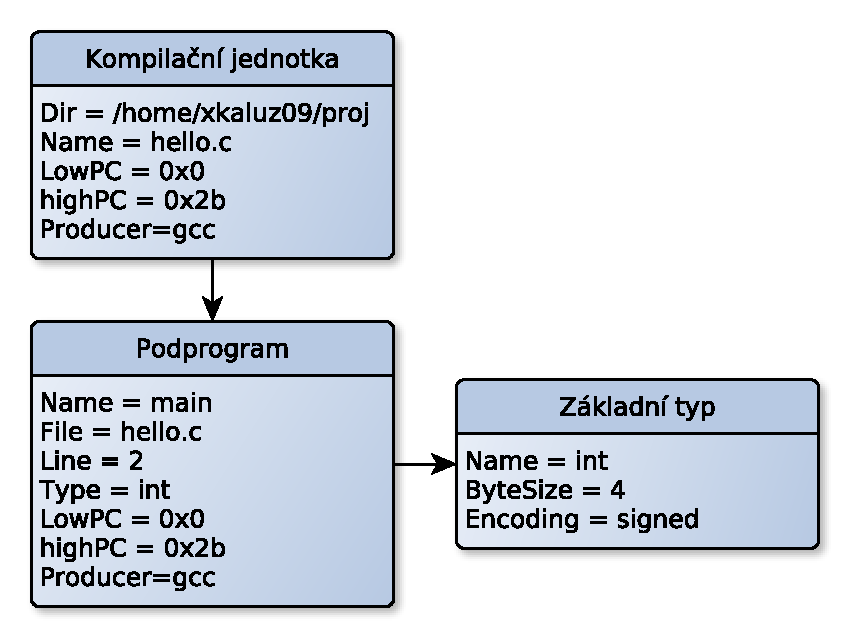
\includegraphics[trim=0cm 0cm 0cm 0cm, scale=0.7]{fig/dwarf}
\caption{DWARF strom Hello World programu v jazyce C.}
\label{fig:dwarf}
\end{figure}

Formát DWARF definuje velké množství typů uzlů a jejich atributů. Z hlediska simulátorů je však důležité popsat ještě uložení proměnných. Proměnné mají krom svého jména a typu ještě lokaci. Ta definuje, kde se nachází hodnota proměnné. Adresa proměnné se však může během běhu programu měnit - někdy bude výhodné mít proměnnou v registru, jindy v paměti, nebo dokonce z části v registru a z části v paměti. Proto je lokace proměnné ve formátu DWARF většinou definována v závislosti na adrese aktuální instrukce v takzvaném seznamu lokací.

Seznam lokací obsahuje pro každou proměnnou její lokaci v závislosti na adrese aktuální instrukce. Každá lokace je pak tvořena kódem zásobníkového automatu se speciálními mikroinstrukcemi, po jehož vykonání je na jeho vrcholu buď samotná hodnota proměnné, číslo registru ve kterém se hodnota nachází nebo
adresa místa v paměti, kde hodnotu najdeme.

K získání těchto informací z ELF souboru lze opět použít nástroj objdump.

\chapter{Událostně řízená simulace}

Událostně řízená simulace modeluje simulovaný systém jako sled diskrétních událostí. Každá událost se odehrává v přesně stanoveném čase a mění celkový
stav systému. Mezi jednotlivými událostmi se stav systému nemění a je tak možné zpracovávat po sobě jdoucí události bez ohledu na časový interval
mezi nimi.

Každá událostně řízená simulace ma svůj globální stav. Ten zahrnuje všechny proměnné a atributy studovaného systému. Globální stav se může v průběhu
simulace měnit vykonáváním událostí. Simulace také udržuje aktuální hodnotu simulačního času pro správné plánování událostí.

Další důležitou částí událostně řízené simulace je seznam událostí. V seznamu jsou události, které ještě nebyly zpracovány. Události jsou seřazeny
vzestupně podle simulačního času. Samotná simulace pak funguje tak, že simulátor změní simulační čas na hodnotu první naplánované události ze seznamu událostí. Tuto událost vykoná a pokračuje další naplánovanou událostí. Každá událost může při svém vykonávání přidávat do seznamu událostí další položky. Simulace končí při dosažení ukončující podmínky (například omezení simulačním časem nebo ukončení simulace při prázdném seznamu událostí).

\section{DEVS}

DEVS (Discrete Event System Specification) je hierarchický a modulární formalismus pro návrh a modelování systémů s diskrétními událostmi.
Základem DEVS je atomický model popisující chování části systému. Je definován jako sedmice:

\begin{math}
M=<X,Y,S,ta, \delta_{ext}, \delta_{int}, \lambda>
\end{math}

\begin{itemize}
\item $X$ - množina vstupních událostí.
\item $Y$ - množina výstupních událostí.
\item $S$ - množina stavů.
\item $ta:S \rightarrow \mathbb{T}^\infty$ - funkce posunu času definující dobu setrvání v daném stavu.
\item $\delta_{ext}:Q \times X \rightarrow  S$ - funkce změny stavu určující jak vstupní událost změní stav systému, kde $Q=\{(s,t_e)|s \in S, t_e \in (\mathbb{T} \cap [0, ta(s)])\}$ je množina všech stavů a $t_e$ je čas uběhlů od poslední události.
\item $\delta_{int}:S \rightarrow S$ je funkce definující změnu stavu systému po uplynutí doby setrvání v daném stavu.
\item $\lambda:S \rightarrow  Y^\phi$ je výstupní funkce, kde $Y^\phi=Y \cup \{\phi\}$ a $\phi \not\in Y$. Tato funkce definuje jak změna stavu systému, po uplynutí doby setrvání v něm, generuje výstupní událost.
\end{itemize}

Atomické modely tedy reagují na vstupní události změnou svého stavu a případně také generováním výstupní události. Svůj stav mohou měnit také samovolně po uplynutí doby setrvání v daném stavu.

Atomické modely je možné dále hiearchicky sdružovat pomocí formalismu Spojovaného DEVS definovaného jako osmice:

\begin{math}
N=<X,Y,D,\{M_i\},C_{xx}, C_{yx}, C_{yy}, Select>
\end{math}

\begin{itemize}
\item $X$ - množina vstupních událostí.
\item $Y$ - množina výstupních událostí.
\item $D$ - množina jmen podkomponent této DEVS komponenty.
\item $M_i$ - množina podkomponent kde pro každou platí $i \in D$.
\item $C_{xx}\subseteq X \times \bigcup_{i \in D} X_i$ - množina externích vstupních propojení.
\item $C_{yx}\subseteq \bigcup_{i \in D} Y_i \times \bigcup_{i \in D} X_i$ - množina interních propojení.
\item $C_{yy}: \bigcup_{i \in D} Y_i \rightarrow Y^\phi$ - množina externích výstupních propojení.
\item $Select:2^D \rightarrow D$ - množina funkcí určující jak vybrat událost z množiny událostí naplánovaných na stejný čas.
\end{itemize}

\chapter{Návrh událostně řízeného simulátoru}
\label{navrh}

Cílem této kapitoly je popsat strukturu navrženého simulátoru, jeho rozhraní pro komunikaci s periferiemi a mikrokontrolery a knihovnu implementující mikrokontroler MSP430. Je zde také zmíněno grafické uživatelské rozhraní simulátoru.

\section{Struktura navrženého simulátoru}

Simulátor bude rozdělen do čtyř navzájem se dopňujících částí - simulační jádro, knihovna simulující MCU MSP430, komponenty rozšiřující simulační jádro a grafické uživatelské rozhraní.

Simulační jádro bude založeno na formalismu Spojovaného DEVS a bude umožňovat propojení všech simulovaných komponent. Komponenty budou atomickými modely formalismu DEVS a budou implementovat chování jednotlivých simulovaných periferií jako například tlačítka, LCD displeje nebo i samotného mikrokontroleru. Mikrokontroler bude vzhledem ke své komplexnosti implementován jako nezávislá knihovna. Grafické uživatelské rozhraní pak zpřístupní všechny funkce simulátoru uživateli.

\section{Návrh simulačního jádra}

Simulační jádro bude sloužit k řízení simulace, přeposílání zpráv mezi komponentami a umožní propojení simulovaných komponent (jednoho mikrokontroleru a více periferií). Každá komponenta bude samostatným modulem a bude mít pevně dané rozhraní pro komunikaci s jinými komponentami vyplývající z atomického modelu formalismu DEVS.

Vstupní a výstupní porty definované ve formalismu DEVS budou představovat jednotlivé piny komponent. Spojení mezi porty pak bude značit spojení jednolivých pinů a zprávy posílané mezi porty budou reprezentovat aktuální napětí na pinech.

Každá komponenta bude schopna následujícího chování:

\begin{itemize}
\item Změnit svůj vnitřní stav na základě změny simulačního času.
\item Změnit svůj vnitřní stav na základě externí události přijaté na vstupní port (typicky na základě zprávy od jiné komponenty).
\item Generovat zprávy na výstupní port.
\end{itemize}

Mikrokontroler bude speciálním rozšířením běžné komponenty poskytujícím navíc přístup ke své paměti, regitrům a kódu programu. To umožní řídit simulaci na základě instrukcí, obsahu paměti a registrů daného mikrokontroléru.  V rámci celé simulace je jen jedna instance mikrokontroleru.

Simulační jádro bude umět komponenty dynamicky načítat aniž by docházelo k jeho jakékoliv úpravě. Návrh je tak velmi obecný a umožní snadné přidávání dalších rozšiřujících komponent nebo i simulaci jiného mikrokontroleru.

% \subsection{Komponenty}
% 
% Komponenta je nejmenší simulovatelná část systému. Komponenty jsou navrženy jako samostatné moduly s pevně daným rozhraním, pomocí kterého komunikují s ostatními komponentami simulace. Návrh je tak velmi obecný a umožňuje přidávání dalších rozšiřujících komponent.
% Návrh počítá se dvěma typy komponent:
% 
% \begin{itemize}
% \item \textbf{Periferie} - Je jakákoliv simulační komponenta, která umí reagovat na zprávy přijímané od jiných periférií, generovat nové zprávy a měnit svůj vnitřní stav na základě simulačního času.
% \item \textbf{Mikrokontroler (MCU)} - Jedná se o speciální případ periferie, která obsahuje paměť, registry a kód programu, který vykonává.
% To umožní řídit simulaci na základě instrukcí, obsahu paměti a registrů daného mikrokontroléru.  V rámci celé simulace je jen jedna instance mikrokontroleru. 
% \end{itemize}
% 
% Každá komponenta (periferie) tak bude schopna následujícího chování:
% 
% \begin{itemize}
% \item Změnit svůj vnitřní stav na základě změny simulačního času.
% \item Změnit svůj vnitřní stav na základě externí události přijaté na vstupní port (typicky na základě zprávy od jiné komponenty).
% \item Generovat zprávy na výstupní port.
% \end{itemize}
% 
% Mikrokontrolery navíc oproti periferiím budou poskytovat následující informace:
% 
% \begin{itemize}
% \item Obsah paměti a registrů.
% \item Disassemblovaný kód běžícího programu.
% \end{itemize}
% 
% Vstupní a výstupní porty definované ve formalismu DEVS budou představovat jednotlivé piny komponent. Spojení mezi porty pak bude značit spojení jednolivých
% pinů a zprávy posílané mezi porty budou reprezentovat aktuální napětí na pinech.

% Na obrázku .... lze vidět ukázku propojení dvou komponent (mikrokontroleru MSP430 a periferie - LED diody). Pokud program mikrokontroleru vygeneruje na svůj 
% výstupní port hodnotu 3.3 (tzv. 3.3 voltu), bude tato zprávy předána na vstupní port LED diody, která na jejím základě změní svůj vnitřní stav (tzv. rozsvítí se).

\section{Návrh knihovny simulující MCU MSP430}

Knihovna simulující mikrokontroler MSP430 je klíčovou částí projektu. Bude umožňovat nahrání uživatelského programu a jeho
následnou simulaci pomocí vykonávání instrukcí a běhu svých dalších interních komponent. Tato simulace bude řízena simulačním jádrem. Knihovna také poskytne grafickému uživatelskému rozhraní přístup ke své paměti a registrům, čímž umožní krokování programů. Bude také nabízet přístup k dalším ladícím informacím jako je například umístění lokálních a globálních proměnných v paměti nebo v registrech s využitím DWARF ladících informací. \cite{cvs}

Na obrázku \ref{fig:msp430_arch} lze vidět základní schéma MSP430 knihovny a její dekompozici. V této podkapitole jsou jednotlivé části tohoto schématu podrobněji rozebrány s důrazem na jejich funkci a postavení v rámci celé MSP430 knihovny.

\begin{figure}[ht]
\centering
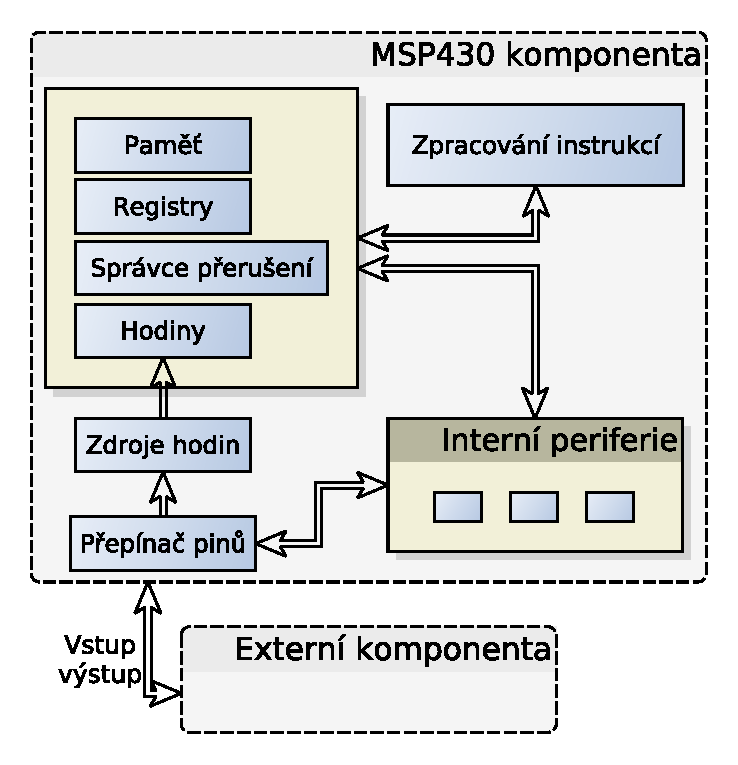
\includegraphics[trim=0cm 0cm 0cm 0cm, scale=0.7]{fig/msp430_arch}
\caption{Návrh architektury MSP430 komponenty.}
\label{fig:msp430_arch}
\end{figure}

\subsection{Paměť}

Paměť slouží k uchování jak uživatelského programu tak dat. Ostatní části mikrokontroleru (zejména pak interní periferie jako například USI nebo USCI) musí být schopny do paměti zapisovat jak slova tak jednotlivé byty a být informovány o případném čtení nebo zápisu provedeném uživatelským programem. To je podstatná vlastnost například pro automatické smazání příznaku přerušení po jeho přečtení. Dalším možným využitím informování o zápisu do paměti je možnost zastavení simulace po změně hodnoty v paměti a tím lepší možnost ladit uživatelský program.

Do paměti musí být umožněno načtení uživatelského programu ve formátu A43. Načítání programu z ELF souboru bude probíhat jeho převodem na formát A43 a následným načtením.

\subsection{Registry}

Návrh registrů, podobně jako návrh paměti, počítá s možností čtení a zápisu jednoho nebo dvou bytů. Opět je potřeba umožnit ostatním částem mikrokontroleru zjistit, že došlo k zápisu do registru. Typickým předpokládaným využitím je krokování programu na základě hodnoty PC registru. Další možné využití může být monitorování stavového registru a zastavení simulace při určitém příznaku.

\subsection{Přepínač pinů}

Každá varianta mikrokontroleru obsahuje různé interní periferie a tím pádem i jiný počet pinů a jejich rozmístění na pouzdru mikrokontroleru. Na jeden pin může být zapojeno více interních periferií a to, která periferie právě daný pin obsluhuje, je určeno na pomocí řídících registrů (například PxSEL a PxSEL2).

Jednotlivé varianty mikrokontroleru MSP430 budou z hlediska pinů a jejich připojení na interní periferie popsány v XML souboru, který bude obsahovat o každém pinu následující informace:

\begin{itemize}
\item Umístění pinu na pouzdru mikrokontroleru (vlevo, vpravo, ...) včetně jeho pořadí na dané straně pouzdra.
\item Seznam názvů vstupů/výstupu realizovaných pomocí pinu a hodnoty bitů v řídících registrech určujících, který vstup/výstup bude kdy zvolen.
\end{itemize}

Interní komponenty (například časovač nebo modul USI) budou mít zaregistrovány v přepínači pinů názvy svých vstupů a výstupů.
Přepínač pinů pak bude na základě aktuálně simulované varianty MSP430 mikrokontroleru monitorovat řídící registry PxSEL, PxSEL2, atd. a podle jejich hodnoty přeposílat vstupy z externích komponent konkrétním interním periferiím (princip multiplexoru). Tento princip ilustruje obrázek \ref{fig:msp430_pinmult}.

\begin{figure}[h]
\centering
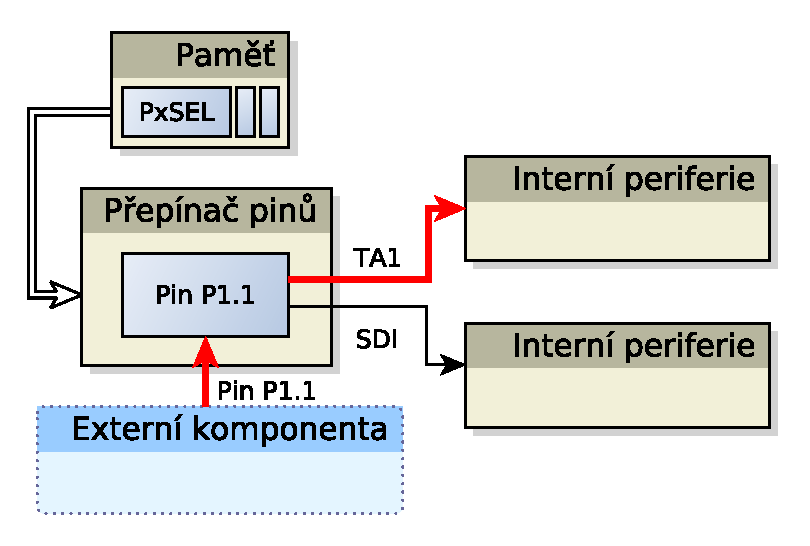
\includegraphics[trim=0cm 0cm 0cm 0cm, scale=0.7]{fig/msp430_pinmult}
\caption{Přepínač pinů přeposílá vstup z externí komponenty na interní periferii podle hodnoty PxSEL.}
\label{fig:msp430_pinmult}
\end{figure}

Přepínač pinů bude rovněž směrovat signály uvnitř MSP430 komponenty. Toho bude potřeba pro interní propojení jednotlivých interních periferií (například výstup časovače může být použit jako vstup modulu USI - toto propojení se děje uvnitř MSP430 komponenty bez využití externích pinů).

\subsection{Zdroje hodin}

Zdroje hodin budou generovat hodinový signál o určité frekvenci. Tento signál pak bude sloužit hodinám (MCLK, SMCLK a ACLK) pro řízení jednotlivých částí mikrokontroleru. Z hlediska simulace je možné zdroje hodin rozdělit na dvě kategorie. Zdroje závislé na externích komponentách (LFXT1CLK, XT2CLK) a zdroje závislé pouze na čase (VLOCLK, DCOCLK).

Zdroje závislé na externích komponentách musí být schopny přijímat zprávy od externích komponent a na jejich základě pak generovat hodinový signál, který je dále zpracován jednotlivými hodinami.

Zdroje závislé na čase musí být samostatnými simulačními komponentami a musí samy na základě uběhnutého času generovat hodinový signál s patřičnou frekvencí.

Všechny zdroje hodin musí generovat informace jak o náběžné, tak o sestupné hraně hodinového signálu. To je podstatná vlastnost například pro modul USI, který provádí své akce jak s oběma hranami hodinového signálu.

\subsection{Hodiny}

Hodiny (MCLK, SMCLK a ACLK) dále zpracovávají hodinový signál od zdrojů hodinového signálu. Umožňují nastavit děličku, čímž mění frekcenci hodinového signálu. K jednotlivým hodinám budou připojeny interní periferie, které jimi budou řízeny. Stejně jako u zdrojů hodinového signálu je potřeba u zdrojů hodin poskytovat informace jak o náběžné tak o sestupné hraně.

\subsection{Správce přerušení}

Správce přerušení bude udržovat informace o požadavcích na přerušení. Modulu zpracovávajícímu instrukce umožní spustit rutinu přerušení, pokud je nějaké
přerušení ve frontě. Ostatním interním komponentám pak umožní žádat o přerušení.

Interní komponenty budou rovněž potřebovat informaci o dokončení konkrétního typu přerušení (například pro vymazání příznaku přerušení po jeho obsluze).

\subsection{Zpracování instrukcí}

Zpracování instrukcí ilustruje diagram na obrázku \ref{fig:msp430_inst}.

\begin{figure}[h]
\centering
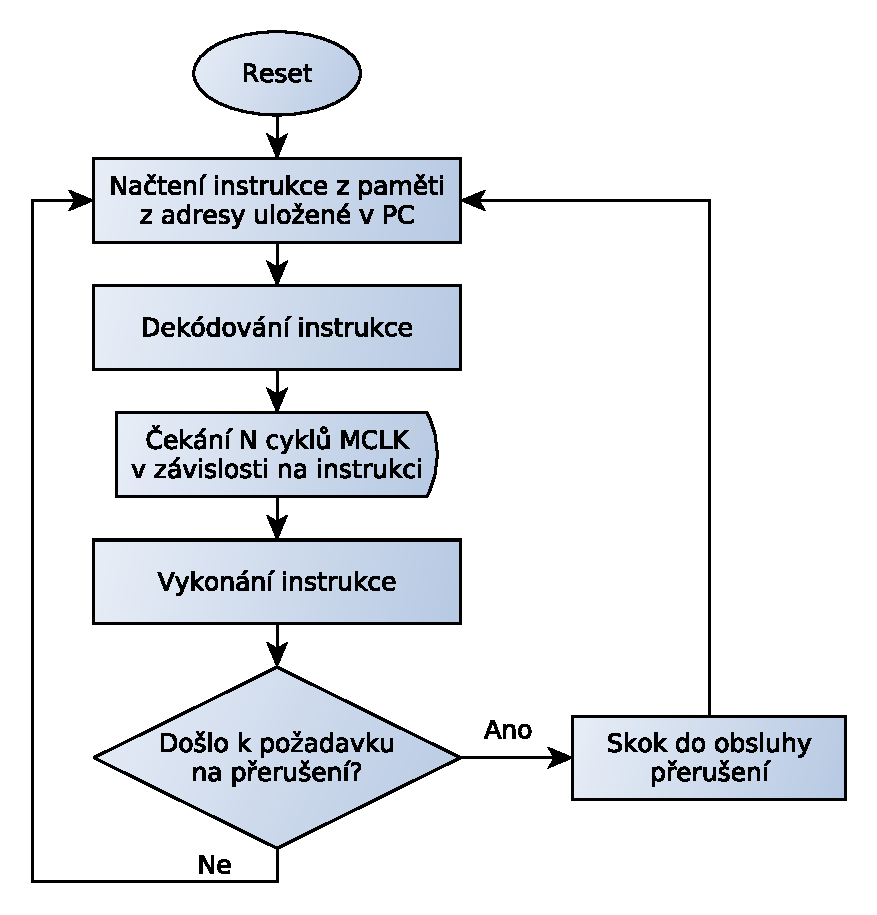
\includegraphics[trim=0cm 0cm 0cm 0cm, scale=0.7]{fig/msp430_inst}
\caption{Diagram zpracování instrukcí.}
\label{fig:msp430_inst}
\end{figure}

Z obrázku lze vidět, že je zpracování instrukce rozděleno na několik částí. Nejprve je instrukce načtena z paměti v závislosti na hodnotě registru PC (R0).
Dále dojde k dekódování instrukce a jejímu vykonání. Vykonání instrukce je atomické a trvá několik MCLK cyklů. Počet cyklů potřebných pro vykonání
instrukce je znám již po jejím dekódování. Proto je mezi dekódováním a vykonáním vloženo čekání simulující vykonávání instrukce na reálném HW.
Po vykonání instrukce je potřeba obsloužit jakákoliv přerušení, která mohla v mezičase nastat. Tento cyklus se bude opakovat stále dokola, dokud MCLK generuje další pulsy (tzv. dokud simulace běží).

\subsection{Interní periferie}

Interní periferie budou využívat modulů popsaných dříve v této kapitole. Každá interní periferie tak bude mít přístup k paměti, registrům, pinům, správci
přerušení a hodinovému signálu. V rámci diplomové práce bude z interních periferií implementován časovač, modul USI a USCI.

Jako příklad návrhu interní periferie se tato podkapitola věnuje pouze časovači. Princip návrhu ostatních periferií je však obdobný, liší se pouze jejich funkcí.

\subsubsection{Časovač}

Časovač bude monitorovat své řídící registry prostřednictvím paměťového modulu a v případě jejich změny, způsobené uživatelským programem, změní také své nastavení (výběr módu, vstupů atd.). Pro generování nastavení Capture overflow bitu (indikace situace, kdy uživatelský program nestihl přečíst hodnotu časovače během 2 přerušení) je potřeba vědět, zda uživatelský program přečetl aktuální hodnotu časovače. To bude řešeno opět pomocí paměťového modulu, kdy tento bude informovat časovač o přečtení dané hodnoty z paměti.

Časovač musí být schopen zvyšovat svoji hodnotu v závislosti na frekvenci. Proto bude časovač napojen na modul hodin (SMLK nebo ACLK). S každým cyklem
hodin pak v závislosti na svém nastavení vykoná danou funkci.

Pomocí časovače lze rovněž generovat pulsy na výstupních pinech umístěných na pouzdře mikrokontroleru a vzorkovat napětí na pinech vstupních.
Je proto nutné umožnit časovači přístup k těmto pinům. To bude provedeno pomocí přepínače pinů. Časovač si zaregistruje potřebné názvy vstupů a výstupů
a přepínač pinů pak v závislosti na akcích uživatelského programu bude směrovat vstupy mikrokontroleru přímo do časovače.

Přerušení časovače jsou generována pomocí správce přerušení. Je však potřeba zajistit, aby se časovač dozvěděl o dokončení rutiny obsluhující přerušení
(přerušení časovače je sdíleno více zdroji přerušení a časovač musí být schopen požádat o další přerušení z jiného zdroje ihned po obsloužení původního přerušení). Toto je zajištěno monitorováním ukončených přerušení pomocí správce přerušení.

Z příkladu časovače lze vidět, že návrh a dekompozice mikrokontroleru MSP430 je dostačující pro interní periferie a poskytuje všechny potřebné vlastnosti.

\section{Návrh grafického uživatelského rozhraní}

Hlavní funkcí grafického uživatelského rozhraní bude řízení simulace, jednoduchá editace jednotlivých simulovaných komponent a lazení programu mikrokontroleru.

Grafické uživatelské rozhraní by tedy mělo mít následující funkce:

\begin{itemize}
\item \textbf{Správa projektu} - Vytvoření, uložení a nahrání projektu.
\item \textbf{Editace projektu} - Přidávání a odebírání simulovaných komponent a editace jejich propojení.
\item \textbf{Řízení simulace} - Nastavení parametrů simulace, kontrola jejího běhu, krokování atd.
\item \textbf{Lazení programu} - Zobrazení zdrojového kódu programu, hodnoty proměnných, registrů, paměti.
\item \textbf{Lazení signálů} - Možnost kontrolovat v čase signály přenášené mezi simulovanými komponentami.
\end{itemize}

V této kapitole jsou tyto požadavky kladené na grafické uživatelské rozhraní detailně rozebrány a je navrženo grafické uživatelské rozhraní, které tyto
požadavky splňuje.

\subsection{Základní koncepce}

Nejdůležitější součástí hlavního okna simulátoru bude kreslící plocha. Na této ploše budou vykresleny jednotlivé simulované komponenty (mikrokontroler
a periferie) včetně jejich pinů a propojení mezi piny. Uživatel bude schopen přidávat nové komponenty a odstraňovat stávající, propojovat je pomocí
vodičů a měnit jejich vlastnosti (například barvu LED diody). Během simulace se budou všechny komponenty aktualizovat a uživatel tak uvidí průběh simulace
(LED dioda bude blikat, aktivní piny budou zobrazeny rozdílnou barvou než piny neaktivní atd.).

Další důležitou částí grafického uživatelského rozhraní bude zobrazení zdrojového kódu programu nahraného v mikrokontroleru. Tento kód bude poskytnut
přímo mikrokontrolerem a GUI jej pouze zobrazí. Z principu lze vždy zobrazit kód v assembleru. Pokud však bude dostupný zdrojový kód v jazyce C, bude 
simulátor schopen přepínat mezi kódem v assembleru a kódem v C. Po zastavení simulace se zobrazí aktuální instrukce (případně odpovídající příkaz v jazyce C). Uživatelské rozhraní bude rovněž umožňovat nastavení breakpointů (bodů zastavení) na jednotlivých instrukcích, čímž umožní jednodušší krokování
simulace.

Pro zobrazení interních informací o jednotlivých simulovaných komponentách bude sloužit třetí část uživatelského rozhraní. Půjde o strukturovaný seznam
typu název-hodnota, který bude zobrazovat informace o aktuálních hodnotách registrech mikroprocesoru, důležitých místech v paměti, nebo například hodnotách
lokálních proměnných v místě zastavení simulace. Každá komponenta bude schopna přidat do tohoto seznamu své položky a předávat tak uživateli potřebné
interní informace.

Poslední dílčí částí uživatelského rozhraní bude rozhraní pro zobrazení napětí na jednotlivých pinech formou osciloskopu. Uživatel si bude moci vybrat
piny, které chce během simulace sledovat a během simulace (nebo i po jejím zastavení) uvidí veškeré změny signálu, které se na pinech odehrály.

\subsection{Správa projektu}

Při vytvoření nového projektu bude uživatel dotázán na vybrání jeho architektury (návrh celé aplikace se neomezuje pouze na mikrokontrolery rodiny MSP430) a varianty dané architektury (v případě mikrokontroleru MSP430 se bude jednat o jeho konkrétní typ). Po vytvoření projektu uvidí uživatel na kreslící ploše vybraný mikrokotroler a bude mu umožněno nahrání programu a přidání dalších periferií.

Při uložení projektu bude potřeba uložit informace o všech komponentách, jejich propojení a umístení na kreslící ploše. Budou se rovněž ukládat informace
o aktuálně používaných breakpointech a sledovaných pinech.

\subsection{Editace projektu}

Editace projektu bude probíhat na kreslící ploše zobrazující všechny komponenty. Na kreslící plochu bude možné přidávat nové periferie ze seznamu periferií, případně ostraňovat periferie stávající. Uživateli bude umožněno periferiemi volně pohybovat po kreslící ploše a propojovat jejich piny pomocí vodičů. Bude možné propojit i více než 2 piny (lze tak vytvořit sběrnicovou topologii s uzly). Propojení mezi piny bude možné odstraňovat.

\subsection{Řízení simulace}

Grafické uživatelské rozhraní umožní spuštění simulace, její dočasné zastavení a její restartování. Během simulace bude uživateli prezentován aktuální simulační čas a uvidí změny simulovaného zapojení na kreslící ploše a osciloskopu. Při dočasném zastavení simulace uvidí uživatel aktuální
stav simulovaného zapojení (stav všech registrů a paměti, následující instrukci ve zdrojovém kódu atd.). Simulaci bude také možné automaticky zastavit po určitém simulačním čase.

K dispozici bude také funkce pro krokování programu s následujícími 3 módy:

\begin{itemize}
\item \textbf{Událost simulace} - Provede další událost v simulaci. Jedná se například o jeden tik hodin MCLK, nebo 1 tik externího oscilátoru. Jedna událost je nejmenší možný krok, jaký lze v diskrétní simulaci provést.
\item \textbf{Instrukce} - Provede další instrukci mikrokontroleru. Instrukce zpravidla trvá více simulačních kroků, půjde tedy o méně jemné krokování simulace.
\item \textbf{Řádek v jazyce C} - Provádí instrukce mikrokontroleru, dokud tyto implementují stále tentýž řádek ve zdrojovém souboru v jazyce C. Při volbě tohoto krokování musí být výsledná aplikace schopna detekovat cykly (například 1 instrukce NOP opakující se stále dokola ve smyčce), aby nedošlo k zamrznutí simulace při vykonávání kroku.
\end{itemize}

Další možností pozastavení simulace jsou takzvané breakpointy. Uživatel musí umět nastavit pozastavení simulace v případě, kdy určitý registr nabyl jím definovanou hodnotu (případně když hodnota v paměti definovaná adresou nabyla konkrétní hodnotu).

\subsection{Lazení programu}

Při každém pozastavení simulace uvidí uživatel aktuální instrukci ve zdrojovém kóu. Kromě samotného zdrojového kódu mu budou zobrazeny, pokud byl nahrán program ve formátu ELF s ladícími symboly, názvy všech zdrojových souborů nahraného programu a všech funkcí v daných souborech. Uživatel bude moci vybrat daný soubor a funkci v něm pro rychlejší orientaci v projektu. V případě dostupnosti zdrojového kódu v jazyce C se uživateli zobrazí jeho kód. Vždy však bude možné zobrazit diassemblovaný kód v assembleru. Uživatel bude moci přidávat breakpointy v libovolných místech kódu a po opětovném spuštění simulace se tato zastaví na místě, které uživatel zvolil.

V grafickém uživatelském rozhraní budou rovněž zobrazeny hodnoty registrů a důležitých adres v paměti (standardně hexadecimálně, avšak bude možné zobrazit jejich hodnoty i v jiných soustavách). Uživatel bude moci použít tento seznam registrů a míst v paměti pro rychlé přidání nových breakpointů. Na základě místa ve zdrojovém kódu, na kterém došlo k pozastavení simulace, budou zobrazeny jména a hodnoty lokálních proměnných.

\subsection{Lazení signálů}

Uživateli bude umožněno vybrání pinů na kreslící ploše a jejich zařazení do seznamu sledovaných pinů. V pruběhu simulace se změny napětí na sledovaných pinech budou ukládat a zobrazovat uživateli v graficky pomocí rozhraní podobného osciloskopu. Uživatel tak uvidí vztahy mezi jednotlivými signály generovanými na pinech v závislosti na čase. Standardně bude rozhraní ukazovat průběh celé simulace. Bude však možné určitý časový úsek přiblížit a získat tak detailnější pohled. Uživatelské rozhraní rovněž umožní export těchto dat.

\chapter{Závěr}
